\chapter{Аналитическая часть}

В данной части формализация объектов сцены, а также анализ существующих алгоритмов построения изображений и выбор
наиболее подходящих из них для выполнения поставленной задачи.

\section{Описание объектов сцены}

Сцена состоит из следующих объектов:

\begin{enumerate}[label=\arabic*.]
    \item \textbf{рельеф местности} --- представляет собой трёхмерную поверхность, описывающую топографию земли;

    \item \textbf{вода} --- визуализация эрозии;

    \item \textbf{точечный источник света} --- представляет собой материальную точку;

    \item \textbf{камера} --- определяет точку зрения наблюдателя в сцене.
\end{enumerate}

\section{Формализация задачи}

Входными данными программного обеспечения являются характеристики источника света, информация о положении камеры и
параметры эрозии почвы. Выходными данными является визуализация водной эрозии рельефа.

Формализация задачи в виде IDEF0 диаграммы приведена на рисунке~\ref{img:ramus}.

\begin{figure}[h]
	\centering
	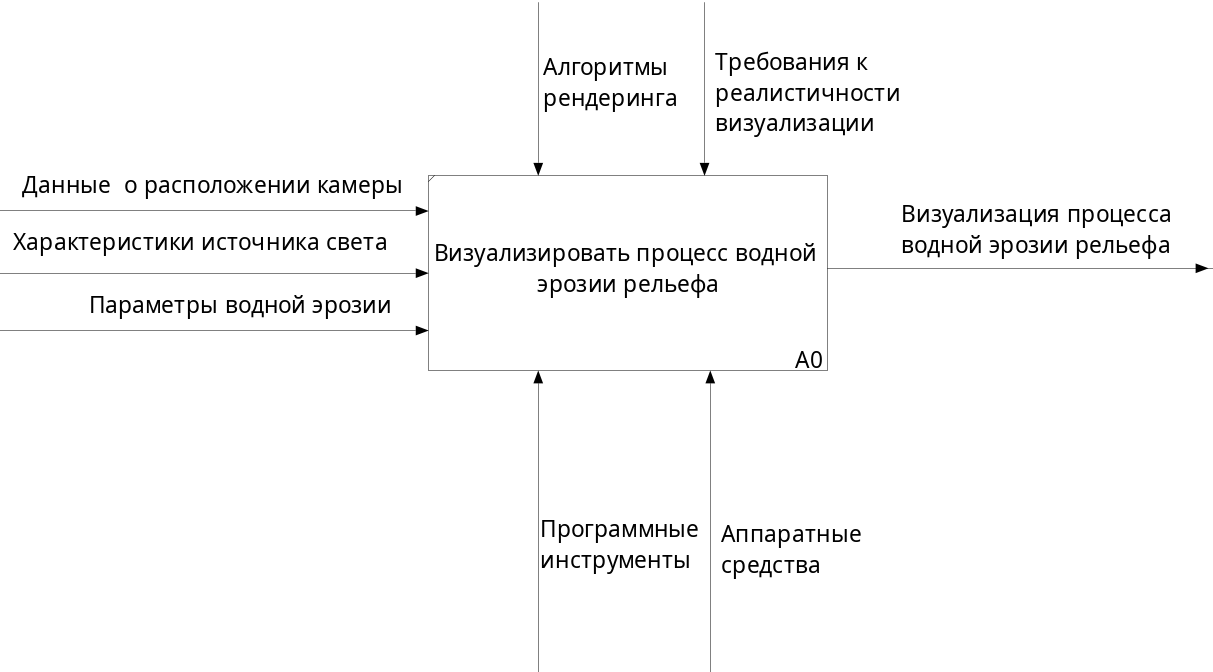
\includegraphics[width=0.8\textwidth]{images/ramus}
	\caption{Формализация задачи в виде IDEF0 диаграммы нулевого уровня}
	\label{img:ramus}
\end{figure}

\subsection{Рельеф местности}

Рельеф местности является ключевым объектом сцены, определяющим основную геометрию и визуальное представление поверхности земли.
Он задаётся высотной картой, представляющей собой двумерный массив, где каждой точке $(x, y)$ соответствует высота $z$.

Для отображения рельефа используется полигональная сетка, состоящая из вершин и граней.
Каждая вершина имеет координаты в трёхмерном пространстве $(x, y, z)$.
Грани в виде треугольников образуются путём соединения вершин.

\subsection{Вода (визуализация эрозии)}

Вода перемещается по поверхности рельефа, взаимодействуя с ним и изменяя его форму путём смыва и переноса частиц грунта.
Это приводит к формированию русел, размыванию склонов и другим эффектам эрозии.

Вода представляется в виде множества капель, скользящих по поверхности.
При движении воды по рельефу учитываются физические параметры, такие как, наклон поверхности.
Сами капли визуального представления не имеют, а только оказывают влияние на рельеф.

\subsection{Источник света}

Основные характеристики источника света:

\begin{itemize}
    \item \textbf{интенсивность} --- определяет яркость света и влияет на освещённость поверхности;
    \item \textbf{положение} --- задаёт координаты источника света в пространстве;
    \item \textbf{цвет} --- описывается компонентами RGB и влияет на оттенок освещения.
\end{itemize}

\subsection{Камера}

Камера определяет точку обзора в сцене и отвечает за проекцию трёхмерного рельефа на двумерный экран.
Параметры камеры включают:

\begin{itemize}
    \item \textbf{положение} --- координаты камеры в трёхмерном пространстве $(x, y, z)$;
    \item \textbf{направление взгляда} --- вектор, определяющий, куда направлена камера;
    \item \textbf{угол обзора} --- определяет поле зрения камеры и влияет на перспективу;
    \item \textbf{параметры проекции} --- параметры ближней и дальней плоскостей отсечения.
\end{itemize}

\clearpage

\section{Способы представления моделей}

В компьютерной графике существует несколько способов представления трёхмерных моделей,
каждый из которых имеет свои преимущества и недостатки. Выбор подходящего метода зависит от требований к визуализации,
производительности и объёму данных.

\subsection{Каркасные модели}

Простейший вид моделей, который содержит информацию только о вершинах и ребрах объектов.
Это моделирование самого низкого уровня, которое имеет ряд серьезных ограничений.
Большинство ограничений возникает из-за недостатка информации
о гранях, которые заключены между ребрами. Невозможно выделить
внутреннюю и внешнюю область изображения твердого объемного тела.
Проблемой этой модели заключается в том, что она
не позволяет отличить видимые грани от невидимых~\cite{rodz}.

\subsection{Поверхностные модели}

Поверхностные модели описывают объект с помощью граней, ограничивающих его форму.
Эти модели позволяют разделить внутреннюю и внешнюю области тела, предоставляя больше возможностей для анализа
и визуализации, чем каркасные.

Поверхностное представление может быть выполнено с использованием многоугольников, чаще всего треугольников,
что делает такие модели удобными для применения текстур и освещения.
Они позволяют визуализировать объект более реалистично, а также обнаруживать пересечения или коллизии между поверхностями.

Такие модели имеют свои ограничения.
Например, они не содержат информации о внутренней структуре объекта.
Кроме того, вычислительная сложность увеличивается с ростом детализации объекта~\cite{rodz}.

\subsection{Объёмные модели}

Объёмные модели описывают объект с учётом его внутренней структуры, предоставляя наиболее полное представление о
форме и содержимом. Для создания таких моделей используются различные подходы, включая воксели (трёхмерные пиксели)
и неявные поверхности, задаваемые математическими функциями~\cite{rodz}.

\subsection{Выбор метода представления моделей}

Для задачи визуализации процесса водной эрозии рельефа необходимо обеспечить отображение изменений поверхности
при сохранении высокой производительности.
Исходя из этого, наиболее подходящими являются поверхностные модели.
Они позволяют эффективно хранить и визуализировать сложный рельеф с высокой детализацией,
необходимой для отображения процессов эрозии.

Недостатки других методов делают их менее пригодными для данной задачи.
Объёмные модели избыточны для визуализации поверхности рельефа,
а простые каркасные модели недостаточны для демонстрации процесса эрозии.

\clearpage

\section{Анализ методов удаления невидимых линий и поверхностей}

Алгоритмы удаления невидимых линий или поверхностей можно классифицировать по способу выбора системы
координат или пространства, в котором они работают. Алгоритмы, работающие в объектном пространстве, имеют дело с
физической системой координат, в которой описаны эти объекты. При этом получаются весьма точные результаты,
ограниченные, вообще говоря, лишь точностью вычислений. Полученные изображения можно свободно увеличивать во много раз.
Алгоритмы, работающие в объектном пространстве, особенно полезны в тех приложениях, где необходима высокая точность.

Алгоритмы же, работающие в пространстве изображения, имеют дело с системой координат того экрана, на котором объекты
визуализируются. При этом точность вычислений ограничена разрешающей способностью экрана~\cite{rodz}.

В данном разделе рассмотрены алгоритм Варнока, Z-буфер, а также методы
прямой и обратной трассировки лучей.

\subsection{Алгоритм Варнока}

Данный алгоритм работает в пространстве изображения. В пространстве изображения
рассматривается окно и решается вопрос о том, пусто ли оно, или его
содержимое достаточно просто для визуализации. Если это не так, то
окно разбивается на фрагменты до тех пор, пока содержимое фрагмента
не станет достаточно простым для визуализации или его размер не
достигнет требуемого предела разрешения~\cite{dem_cg}.

Пример разбиения окна показан на рисунке~\ref{img:varnok}.

\begin{figure}[H]
	\centering
	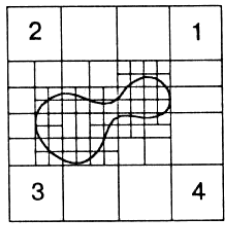
\includegraphics[scale=0.6]{images/varnok}
	\caption{Пример разбиения окна в алгоритме Варнока}
	\label{img:varnok}
\end{figure}

\subsection{Алгоритм, использующий Z буфер}

Одним из самых простых алгоритмов удаления невидимых граней и поверхностей
является метод Z-буфера (буфера глубины). Алгоритм работает в пространстве изображения.
В силу крайней простоты этого метода часто
встречаются его аппаратные реализации~\cite{cg_shik}.

Размеры Z-буфера равны размерам окна, таким образом, каждому пикселю
окна соответствует ячейка Z-буфера. В этой ячейке хранится значение глубины
пикселя. Перед растеризацией сцены Z-буфер заполняется значением,
соответствующим максимальной глубине. В случае, когда глубина характеризуется
значением w, максимальной глубине соответствует нулевое значение.

Анализ видимости происходит при растеризации граней, для каждого пикселя рассчитывается
глубина и сравнивается со значением в Z-буфере, если рисуемый пиксель ближе
(его w больше значения в Z-буфере), то пиксель рисуется, а значение в Z-буфере
заменяется его глубиной. Если пиксель дальше, то пиксель не рисуется и Z-буфер
не изменяется, текущий пиксель дальше того, что нарисован ранее, а значит, невидим~\cite{dem_cg}.

Пример организации Z-буфера показан на рисунке~\ref{img:zbuf}.

\begin{figure}[H]
	\centering
	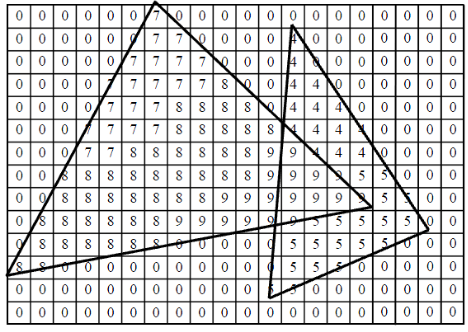
\includegraphics[scale=0.6]{images/zbuf}
	\caption{Пример организации Z-буфера}
	\label{img:zbuf}
\end{figure}

\subsection{Прямая и обратная трассировка лучей}

В этом алгоритме для удаления скрытых линий и поверхностей можно
использовать тот факт, что в реальной природе источник света
испускает луч света, который, «путешествуя» по пространству, в
конечном счете «натыкается» на какую-либо преграду, которая
прерывает распространение этого светового луча. В какой-либо точке
пути с лучом света может случиться любая комбинация трех вещей:
поглощение, отражение (рефлекция) и преломление (рефракция)~\cite{dem_cg}.

\subsubsection{Прямая трассировка лучей}

Суммарная интенсивность светового луча, которая была «потеряна»
вследствие поглощения, преломления и отражения, должна быть в
точности равной исходящей (начальной) интенсивности этого луча.
Далее отраженные и/или преломленные лучи достигают других
поверхностей, где их поглощающие, отражающие и преломляющие
способности снова вычисляются, основываясь на результатах
вычислений входящих лучей. Таким образом, луч, пропущенный через
пиксель картиной плоскости, образует сложный разделяющийся путь~\cite{dem_cg}.

\subsubsection{Обратная трассировка лучей}

Если проследить за лучами света, выпущенным
источником света, то можно убедиться, что весьма немногие дойдут до
наблюдателя. Следовательно, этот процесс вычислительно
неэффективен. Поэтому было предложено отслеживать (трассировать)
лучи в обратном направлении, т.е. от наблюдателя к объекту и далее к
источнику освещения. При этом, интенсивность в пикселе,
через который проходит луч, рассчитывалась бы интегрально с учетом
всех слагаемых: пересечения, отражения, преломления луча с разными
объектами и характеристик источников света. Такой подход получил
название метод обратной трассировки лучей~\cite{dem_cg}.

\subsection{Выбор метода удаления невидимых линий и поверхностей}

Z-буфер является подходящим решением для данной задачи, так как он обрабатывает каждую грань и каждый пиксел независимо,
обеспечивая линейную зависимость времени выполнения от количества объектов в сцене.
Это позволяет программе эффективно справляться с изменениями геометрии рельефа, которые происходят в реальном времени.

В отличие от алгоритмов, таких как прямая и обратная трассировка лучей,
которые требуют сложных геометрических вычислений или предварительной сортировки полигонов,
Z-буфер позволяет обновлять изображение сцены без значительных вычислительных затрат.

\clearpage

\section{Анализ методов закраски}

Световая энергия, падающая на поверхность от источника света, может быть поглощена,
отражена и пропущена.
Свойства отраженного света зависят от формы и направления источника света, а также от
ориентации освещаемой поверхности и ее свойств.
Свет, отраженный от объекта, может быть
диффузным и зеркальным: диффузно отраженный свет рассеивается равномерно по всем
направлениям, зеркальное отражение происходит от внешней поверхности объекта~\cite{cg_shik}.

Диффузное отражение присуще матовым поверхностям. Матовой можно считать такую поверхность,
размер шероховатостей которой уже настолько велик, что
падающий луч рассеивается равномерно во все стороны. Такой тип отражения характерен, например, для гипса, песка, бумаги.
Диффузное отражение описывается законом Ламберта, согласно которому интенсивность отраженного света
пропорциональна косинусу угла между направлением на точечный источник света и нормалью к поверхности~\ref{eq:Lambert}.

\begin{equation}
    \label{eq:Lambert}
    I_{d} = I \cdot K_{d} \cdot \cos{\theta},
\end{equation}

где $I$ — интенсивность источника света, $K_{d}$ — коэффициент, который учитывает свойства материала поверхности~\cite{perm_cg}.

В задаче эрозии рельефа все поверхности являются матовыми.
Поэтому в данном случае достаточно использовать диффузное отражение.

Существует три основных способа закраски объектов, заданных
полигональными сетками. В порядке возрастания сложности ими
являются~\cite{dem_cg}:

\begin{enumerate}
    \item однотонная закраска;
    \item метод Гуро (основан на интерполяции значений интенсивности);
    \item метод Фонга (основан на интерполяции векторов нормали).
\end{enumerate}

\subsection{Однотонная закраска}

Пусть $\vec{L}$ -- вектор, направленный от центра поверхности на точечный источник света, $\vec{N}$ -- нормаль к
поверхности, $\vec{V}$ -- вектор, направленный от центра поверхности к точке зрения (камере).

При однотонной закраске вычисляют один уровень интенсивности,
который используется для закраски всего многоугольника. При этом
предполагается, что:

\begin{enumerate}
    \item источник света расположен в бесконечности, поэтому произведение $\vec{L} \cdot \vec{N}$ постоянно на всей полигональной грани;
    \item наблюдатель находится в бесконечности, поэтому произведение $\vec{N} \cdot \vec{V}$ постоянно на всей полигональной грани;
    \item многоугольник представляет реальную моделируемую поверхность, а не является аппроксимацией криволинейной поверхности.
\end{enumerate}

Если какое-либо из первых двух предположений оказывается неприемлемым, можно воспользоваться усредненными
значениями $\vec{L}$ и $\vec{V}$, вычисленными, например, в центре многоугольника~\cite{dem_cg}.

\subsection{Метод Гуро}

Этот метод позволяет
устранить дискретность изменения интенсивности. Процесс закраски по
методу Гуро осуществляется в четыре этапа~\cite{dem_cg}:

\begin{enumerate}
    \item вычисляются нормали ко всем полигона;
    \item определяются нормали в вершинах путем усреднения нормалей по всем полигональным граням, которым принадлежит вершин;
    \item используя нормали в вершинах и применяя произвольный метод закраски, вычисляются значения интенсивности в вершинах;
    \item каждый многоугольник закрашивается путем линейной интерполяции значений интенсивностей в вершинах сначала вдоль каждого ребра, а затем и между ребрами вдоль каждой сканирующей строки.
\end{enumerate}

\subsection{Метод Фонга}

В методе закраски, разработанном Фонгом, используется
интерполяция вектора нормали N к поверхности вдоль видимого
интервала на сканирующей строке внутри многоугольника, а не
интерполяция интенсивности. Интерполяция выполняется между
начальной и конечной нормалями, которые сами тоже являются
результатами интерполяции вдоль ребер многоугольника между
нормалями в вершинах. Нормали в вершинах, в свою очередь,
вычисляются так же, как в методе закраски, построенном на основе
интерполяции интенсивности~\cite{dem_cg}.

\subsection{Выбор метода закраски}

Для реализации программы по визуализации процесса водной эрозии рельефа был выбран метод закраски по Гуро.
Закраска по Гуро позволяет получить плавные переходы цвета между вершинами полигонов,
что достаточно для визуального восприятия рельефа как непрерывной поверхности.

%Более сложные методы, такие как закраска по Фонгу, нецелесообразны из-за их высокой вычислительной сложности,
%которая может привести к значительным затратам ресурсов и снижению частоты кадров при визуализации.
%Однотонная закраска, при которой цвет полигона вычисляется только один раз для всей его площади, не подходит для
%данной задачи, так как приводит к визуально грубому и нереалистичному отображению рельефа.

\section{Анализ методов визуализации водной эрозии рельефа}

Процесс
водной эрозии почв состоит из разрушения
почв каплями дождя и потоками воды, сформировавшиеся на поверхности склона в результате выпадения дождя
(природных, искусственных) или таяния снега, транспортировке почвенных частиц и агрегатов и их отложения\cite{err}.


Существует несколько подходов к симуляции эрозии, каждый из которых имеет свои особенности.
В данном разделе рассматривается два основных метода.

\subsection{Карта воды}

В данном подходе ландшафт (высотная карта) дополняется двумя дополнительными картами (или слоями):

\begin{itemize}
\item карта воды — хранит, сколько воды находится над каждой ячейкой высотной карты;
\item карта осадка — хранит, сколько грунта (осадка) переносит или содержит вода в каждой ячейке.
\end{itemize}

Итерационно выполняются следующие стадии:

\begin{enumerate}
\item добавление воды (дождь) — во все или выбранные ячейки «льётся» некоторое количество воды;
\item сток воды — каждая ячейка пытается «передать» воду в соседние ячейки, которые ниже по высоте (с учётом уже имеющейся в них воды);
\item эрозия и перенос осадка — при стоке вода «смывает» часть грунта и добавляет его в карту осадка; если скорость потока или уклон недостаточны, осадок может выпасть обратно на поверхность;
\item испарение — часть воды испаряется из каждой ячейки, оставляя отложенный осадок в виде изменения высот.
\end{enumerate}

\subsection{Капельный метод}

Вместо заполненной всей карты водой, здесь эрозия представляется в виде отдельных капель, которые:

\begin{enumerate}
\item создаются в некоторой точке ландшафта с начальным объёмом воды;
\item скользят по рельефу, каждый раз перемещаясь к соседу с более низкой высотой, постепенно смывая грунт;
\item в капле хранится «количество осадка», которое может быть отложено, если капля достигла локальной ямки;
\item капля испаряется или прекращает движение, когда вода в ней заканчивается или когда уклон исчезает.
\end{enumerate}

Процесс повторяется для большого числа капель в разных точках карты.

\subsection{Выбор метода эрозии}

Для решения задачи формирования реалистичных русел, оврагов и направленного переноса грунта наиболее
предпочтительным оказывается «капельный» метод, поскольку он позволяет моделировать локальные потоки воды и точечный
процесс переноса осадка, тогда как «глобальная» карта воды приводит к избыточно равномерному размягчению
рельефа и недостаточно ярко выраженным формам.

\section*{Вывод}

В ходе аналитической части было принято решение представить рельеф в виде полигональной поверхностной модели. Для отсечения
невидимых граней будет использован алгоритм Z-буфера, для закраски выбран метод Гуро, а для эрозии -- капельный метод